\begin{flushright} {\tiny {\color{gray} (tikz\_cr\_3.tex)}} \end{flushright}
%~~~~~~~~~~~~~~~~~~~~~~~~~~~~~~~~~~~~~~~~~~~~~~~~~~~~~~~~~~~~~~~~~~~~~~~~~~~~~~~~~~~~~~~~~~~~~~~~~~


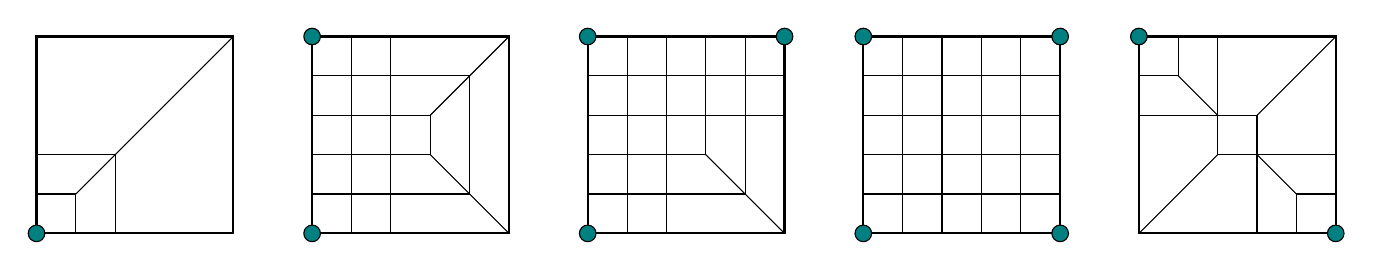
\begin{tikzpicture}
%\draw[step=0.5cm,gray,very thin] (0,0) grid (17,5); %background grid


\draw[thick] (0.5,0.5) rectangle (3,3);
\draw[](0.5,1)--(1,1)--(1,0.5);
\draw[](0.5,1.5)--(1.5,1.5)--(1.5,0.5);
\draw[](1,1)--(3,3);
\draw[black,fill=teal] (0.5,0.5) circle (3pt);


\draw[thick] (4,0.5) rectangle (6.5,3);
\draw[](4.5,0.5)--(4.5,3);
\draw[](5,0.5)--(5,3);
\draw[](4,1.5)--(5.5,1.5)--(5.5,2)--(4,2);
\draw[](4,1)--(6,1)--(6,2.5)--(4,2.5);
\draw[](5.5,2)--(6.5,3);
\draw[](5.5,1.5)--(6.5,0.5);
\draw[black,fill=teal] (4,0.5) circle (3pt);
\draw[black,fill=teal] (4,3) circle (3pt);

\draw[thick] (7.5,0.5) rectangle (10,3);
\draw[](8,0.5)--(8,3);
\draw[](8.5,0.5)--(8.5,3);
\draw[](7.5,2.5)--(10,2.5);
\draw[](7.5,2)--(10,2);
\draw[](7.5,1.5)--(9,1.5)--(9,3);
\draw[](7.5,1)--(9.5,1)--(9.5,3);
\draw[](9,1.5)--(10,0.5);
\draw[black,fill=teal] (7.5,0.5) circle (3pt);
\draw[black,fill=teal] (7.5,3) circle (3pt);
\draw[black,fill=teal] (10,3) circle (3pt);

\draw[thick] (11,0.5) rectangle (13.5,3);
\draw[](11,1)--(13.5,1);
\draw[](11,1.5)--(13.5,1.5);
\draw[](11,2)--(13.5,2);
\draw[](11,2.5)--(13.5,2.5);
\draw[](11.5,0.5)--(11.5,3);
\draw[](12,0.5)--(12,3);
\draw[](12.5,0.5)--(12.5,3);
\draw[](13,0.5)--(13,3);
\draw[black,fill=teal] (11,0.5) circle (3pt);
\draw[black,fill=teal] (11,3) circle (3pt);
\draw[black,fill=teal] (13.5,3) circle (3pt);
\draw[black,fill=teal] (13.5,0.5) circle (3pt);

\draw[thick] (14.5,0.5) rectangle (17,3);
\draw[black,fill=teal] (14.5,3) circle (3pt);
\draw[black,fill=teal] (17,0.5) circle (3pt);
\draw[](14.5,0.5)--(15.5,1.5);
\draw[](16,2)--(17,3);
\draw[](15.5,1.5) rectangle (16,2);
\draw[](14.5,2.5)--(15,2.5)--(15,3);
\draw[](14.5,2)--(15.5,2)--(15.5,3);
\draw[](15,2.5)--(15.5,2);
\draw[](16,1.5)--(16.5,1);
\draw[](16.5,0.5)--(16.5,1)--(17,1);
\draw[](16,0.5)--(16,1.5)--(17,1.5);

\end{tikzpicture}


